\section{Introduction}
\label{sec:introduction}
Joint 4D reconstruction of human-object interaction (HOI) from a monocular video has garnered significant attention in various applications such as immersive AR/VR experiences, robot manipulation, and digital content creation.
This human-object interaction is expressed not only through physical relationships, such as contact between human and object surfaces, but also through high-level semantic relationships that characterize the functional intent of the interaction, such as playing a guitar.
Capturing both relationships from a monocular video is crucial for faithful 4D reconstruction.


While recent approaches for joint human and object reconstruction from a monocular video~\cite{xu2021d3d,xie2023visibility,xue2026rhino,xie2026cari4d,wen2025efficient} have shown notable progress, they still face two main challenges. 
First, their methods rely heavily on geometric proximity, specifically human-object contact, which addresses only local interactions and cannot represent the full range of real-world interactions.
This limitation motivates the use of text descriptions~\cite{nam2026tehor} to reason about the semantic context of the interaction.
However, a video typically contains composite semantic context spanning multiple sub-actions, and summarizing them into a single description makes it difficult to capture which interaction context applies at each moment.
Second, a monocular observation suffers from severe occlusion, where the human and object frequently obscure each other during the interaction.
This lack of geometric cues makes their spatial relationship difficult to reconstruct, often leading to severe interpenetration and temporally inconsistent results.


\begin{figure}[t!]
  \centering
  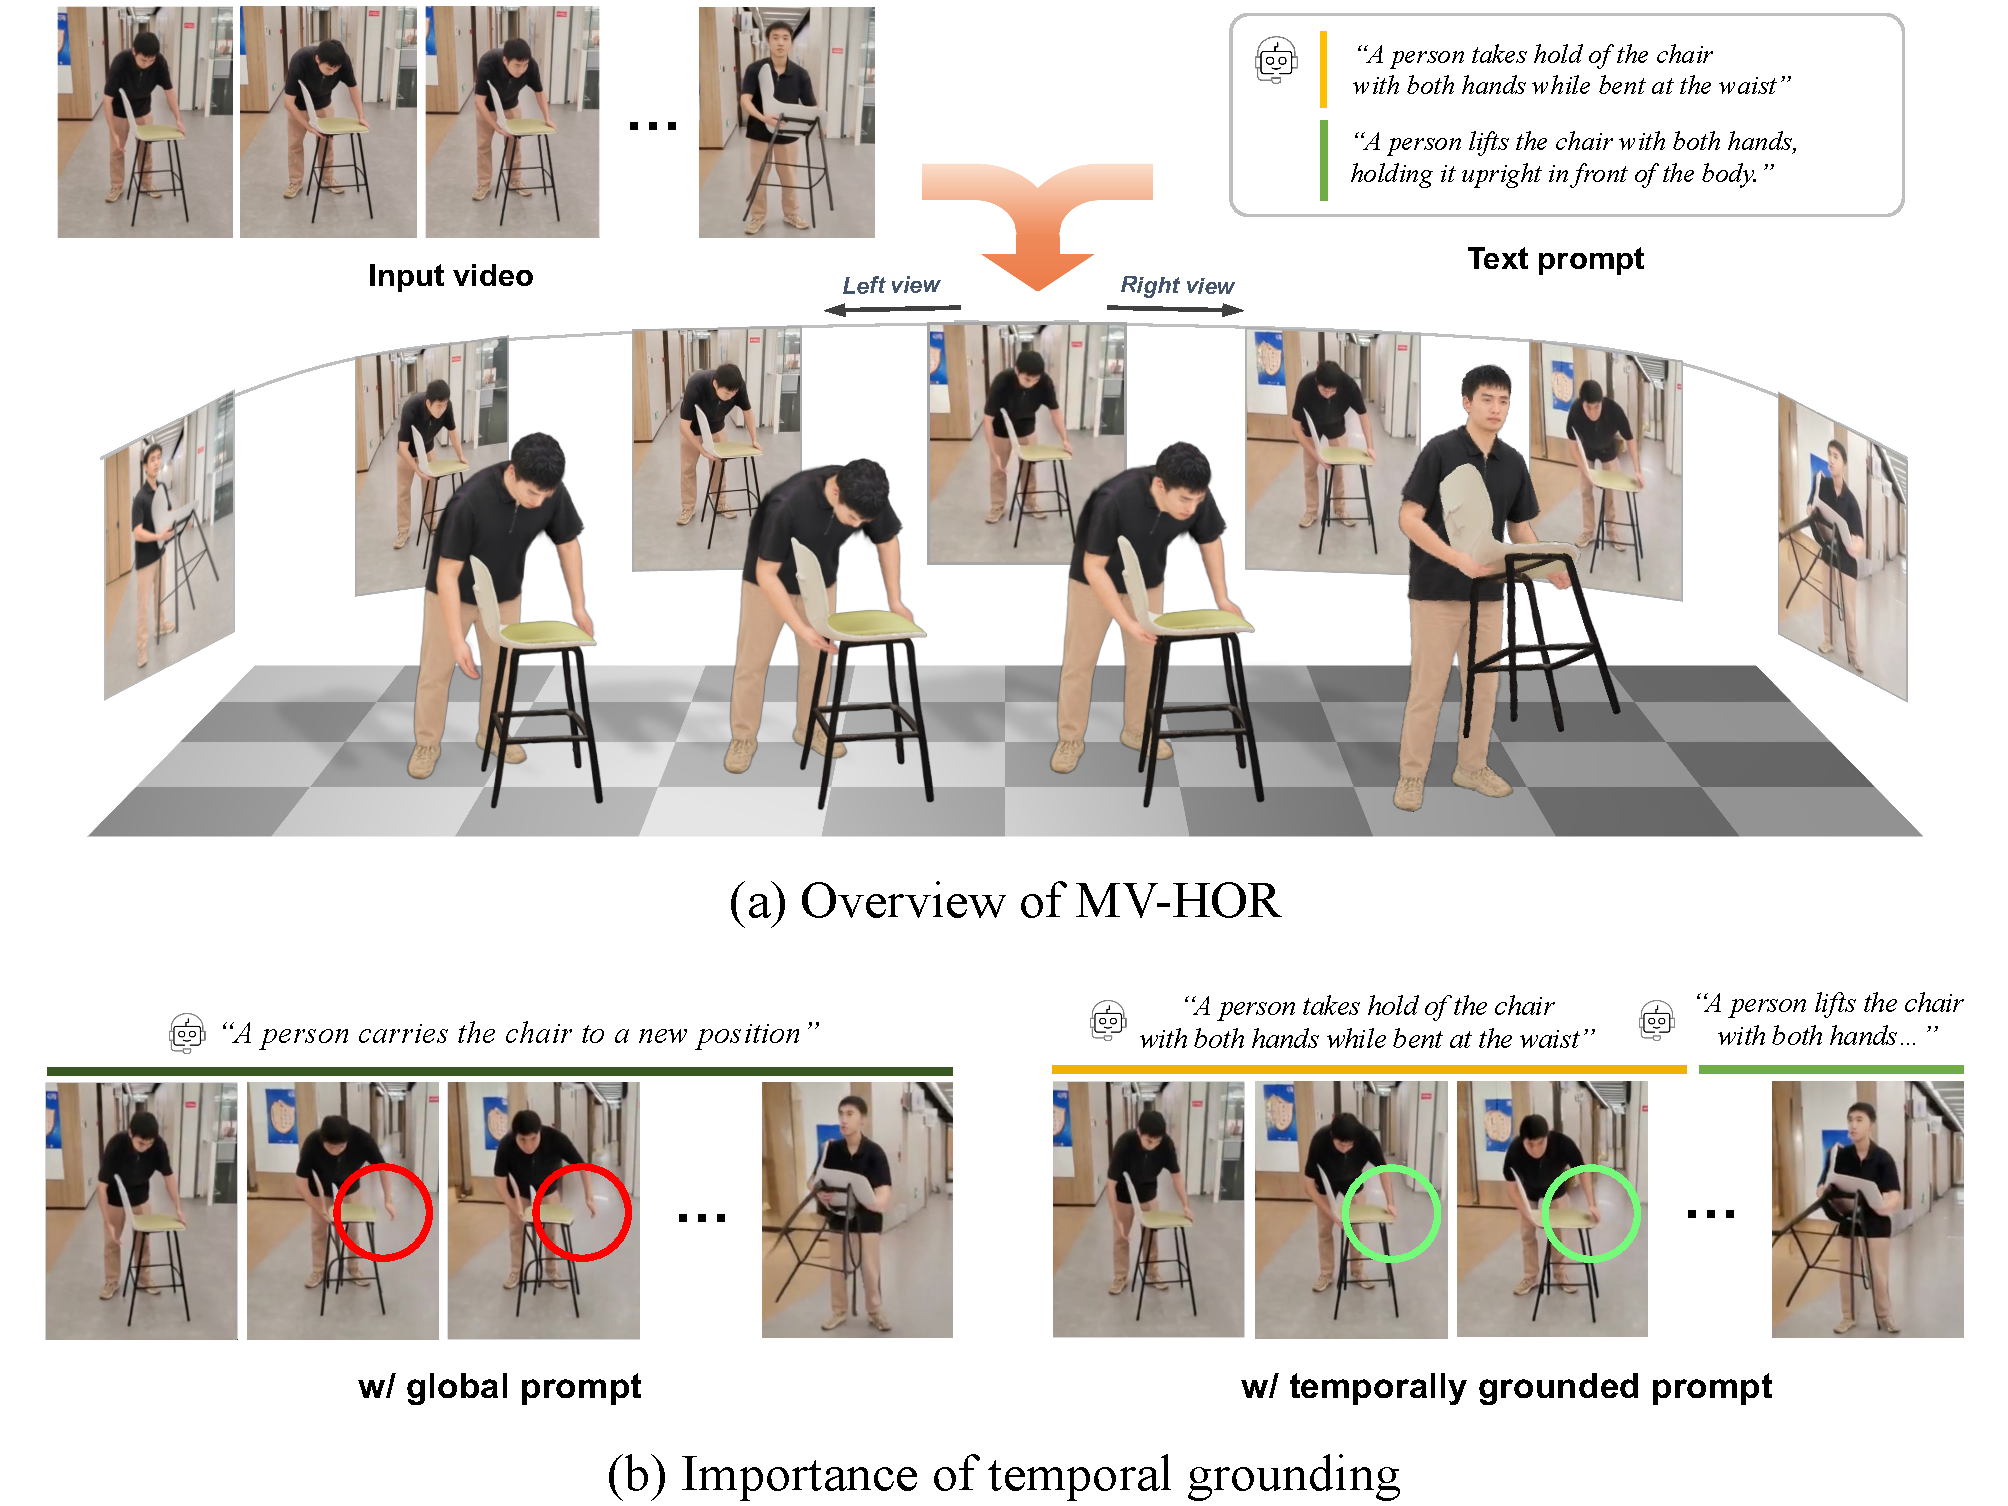
\includegraphics[width=1.0\linewidth]{figures/1_introduction.pdf}
  \vspace*{-1.5em}
  \caption{\textbf{\ourmethod.}
  (a) Overview of our framework.
  (b) Without temporal grounding, the global prompt cannot cover the details of human and object poses, whereas temporally grounded prompts precisely describe them for each interval and enable reliable generation of occluded regions.
  }
  \vspace*{-0.0em}
  \label{fig:1_introduction}
\end{figure}


To address the above challenges, we present \textbf{\ourmethod}, a framework that reconstructs 4D human-object interaction from a monocular video through temporally grounded novel-view video generation.
Our framework first splits the input video into sub-actions and assigns a text description to each segment.
This decomposition is important for capturing fine-grained temporal dynamics throughout the entire interaction sequence.
For example, without temporal decomposition, a single prompt describing the entire video causes the text-to-video model~\cite{wan2025wan} to miss interaction details, such as the contact between the hands and the chair shown in~\cref{fig:1_introduction}~(b).
To decide where to decompose, we first estimate the object motion and incorporate it into the captioning of human-object interactions in the input video, a process we refer to as motion-aware captioning.
Based on each caption, we split the video into temporally grounded sub-actions with precise boundaries.
This temporal grounding facilitates the capture of fine-grained interaction details in text-to-video generation, as shown in \cref{fig:1_introduction}~(b).


Building upon these grounded descriptions, we introduce an interaction-aware re-rendering pipeline to generate novel-view videos that compensate for limited single-view observations in 4D reconstruction.
Specifically, we first render the initially reconstructed human and object from novel viewpoints and refine the renderings with a text-to-video diffusion network~\cite{wan2025wan} that contains rich prior knowledge of human-object interactions learned from large-scale video data.
During this refinement process, we apply distinct text prompts to the human and object regions, each extracted from the text description of the sub-action.
This regional text conditioning guides the video diffusion network to keep the human and object appearances faithful to their own descriptions while specifying where they interact.
With our re-rendering process, we aggregate the refined novel-view videos to provide auxiliary supervision for joint 4D human and object reconstruction.
As a result, our framework accurately reconstructs 4D human-object interactions that follow the semantic context of each sub-action, while ensuring geometric consistency across viewpoints.


Our extensive experiments demonstrate that \ourmethod~significantly outperforms existing reconstruction methods across various interaction scenarios.
Our contributions can be summarized as follows.
\begin{itemize}
\item We propose \textbf{\ourmethod}, a framework for joint 4D reconstruction of a human and object from a monocular video via temporally grounded novel-view video generation.
\item To capture fine-grained human-object interactions across the entire video sequence, we decompose the input video into temporally grounded sub-actions with our proposed motion-aware video captioning.
\item To compensate for limited single-view cues from the input video, we introduce an interaction-aware re-rendering pipeline that provides auxiliary novel-view supervision for accurate 4D human and object reconstruction.
\end{itemize}   

